\chapter{Introduction}\label{sec:introduction}

\section{The IDSC Cubli}\label{sec:cubli}

\begin{figure}[ht]
   \centering
   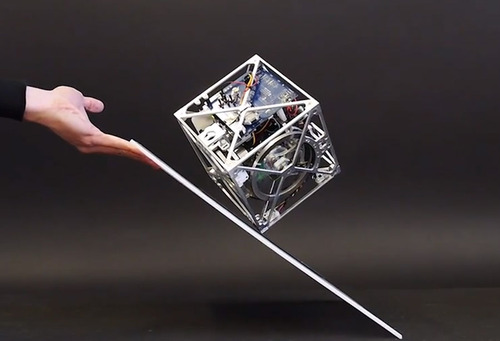
\includegraphics[width=0.75\textwidth]{img/Cubli.jpg}
   \caption{The IDSC Cubli balancing on a slanted surface.}
   \label{img:Cubli}
\end{figure}

The Cubli is a robotic cube developed in the IDSC lab of ETH Zurich, with the ability to balance on its edges and corners by using internal reaction wheels. Of relatively small size (dimensions of 15 x 15 x 15 cm according to \cite{cubliECC13}), the robot is a proof-of-concept made possible through innovative design and engineering.\\

On top of its ability to balance, Cubli is also able to jump through well-timed braking of the reaction wheels. It can thus jump from a face to an edge, a corner, or from a face directly to the corner. It is also able to spin, and stop spinning when balancing on a corner.

\begin{figure}[ht]
   \centering
   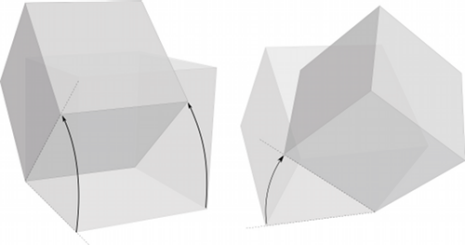
\includegraphics[width=0.75\textwidth]{img/Jumps.png}
   \caption{Illustration of Cubli's jumping abilities.}
   \label{img:Jumps}
\end{figure}

\subsection{Original Interface}
 
Actions can be executed by pressing buttons visible on one of Cubli's faces ( \textit{see Figure \ref{img:Buttons}} ). For example, pressing the Mode button once while holding Cubli on its edge at a stable angle will cause it to start balancing. Or, when Cubli is on its face, press the mode button once and it jumps up to its edge.\\

\begin{figure}[ht]
   \centering
   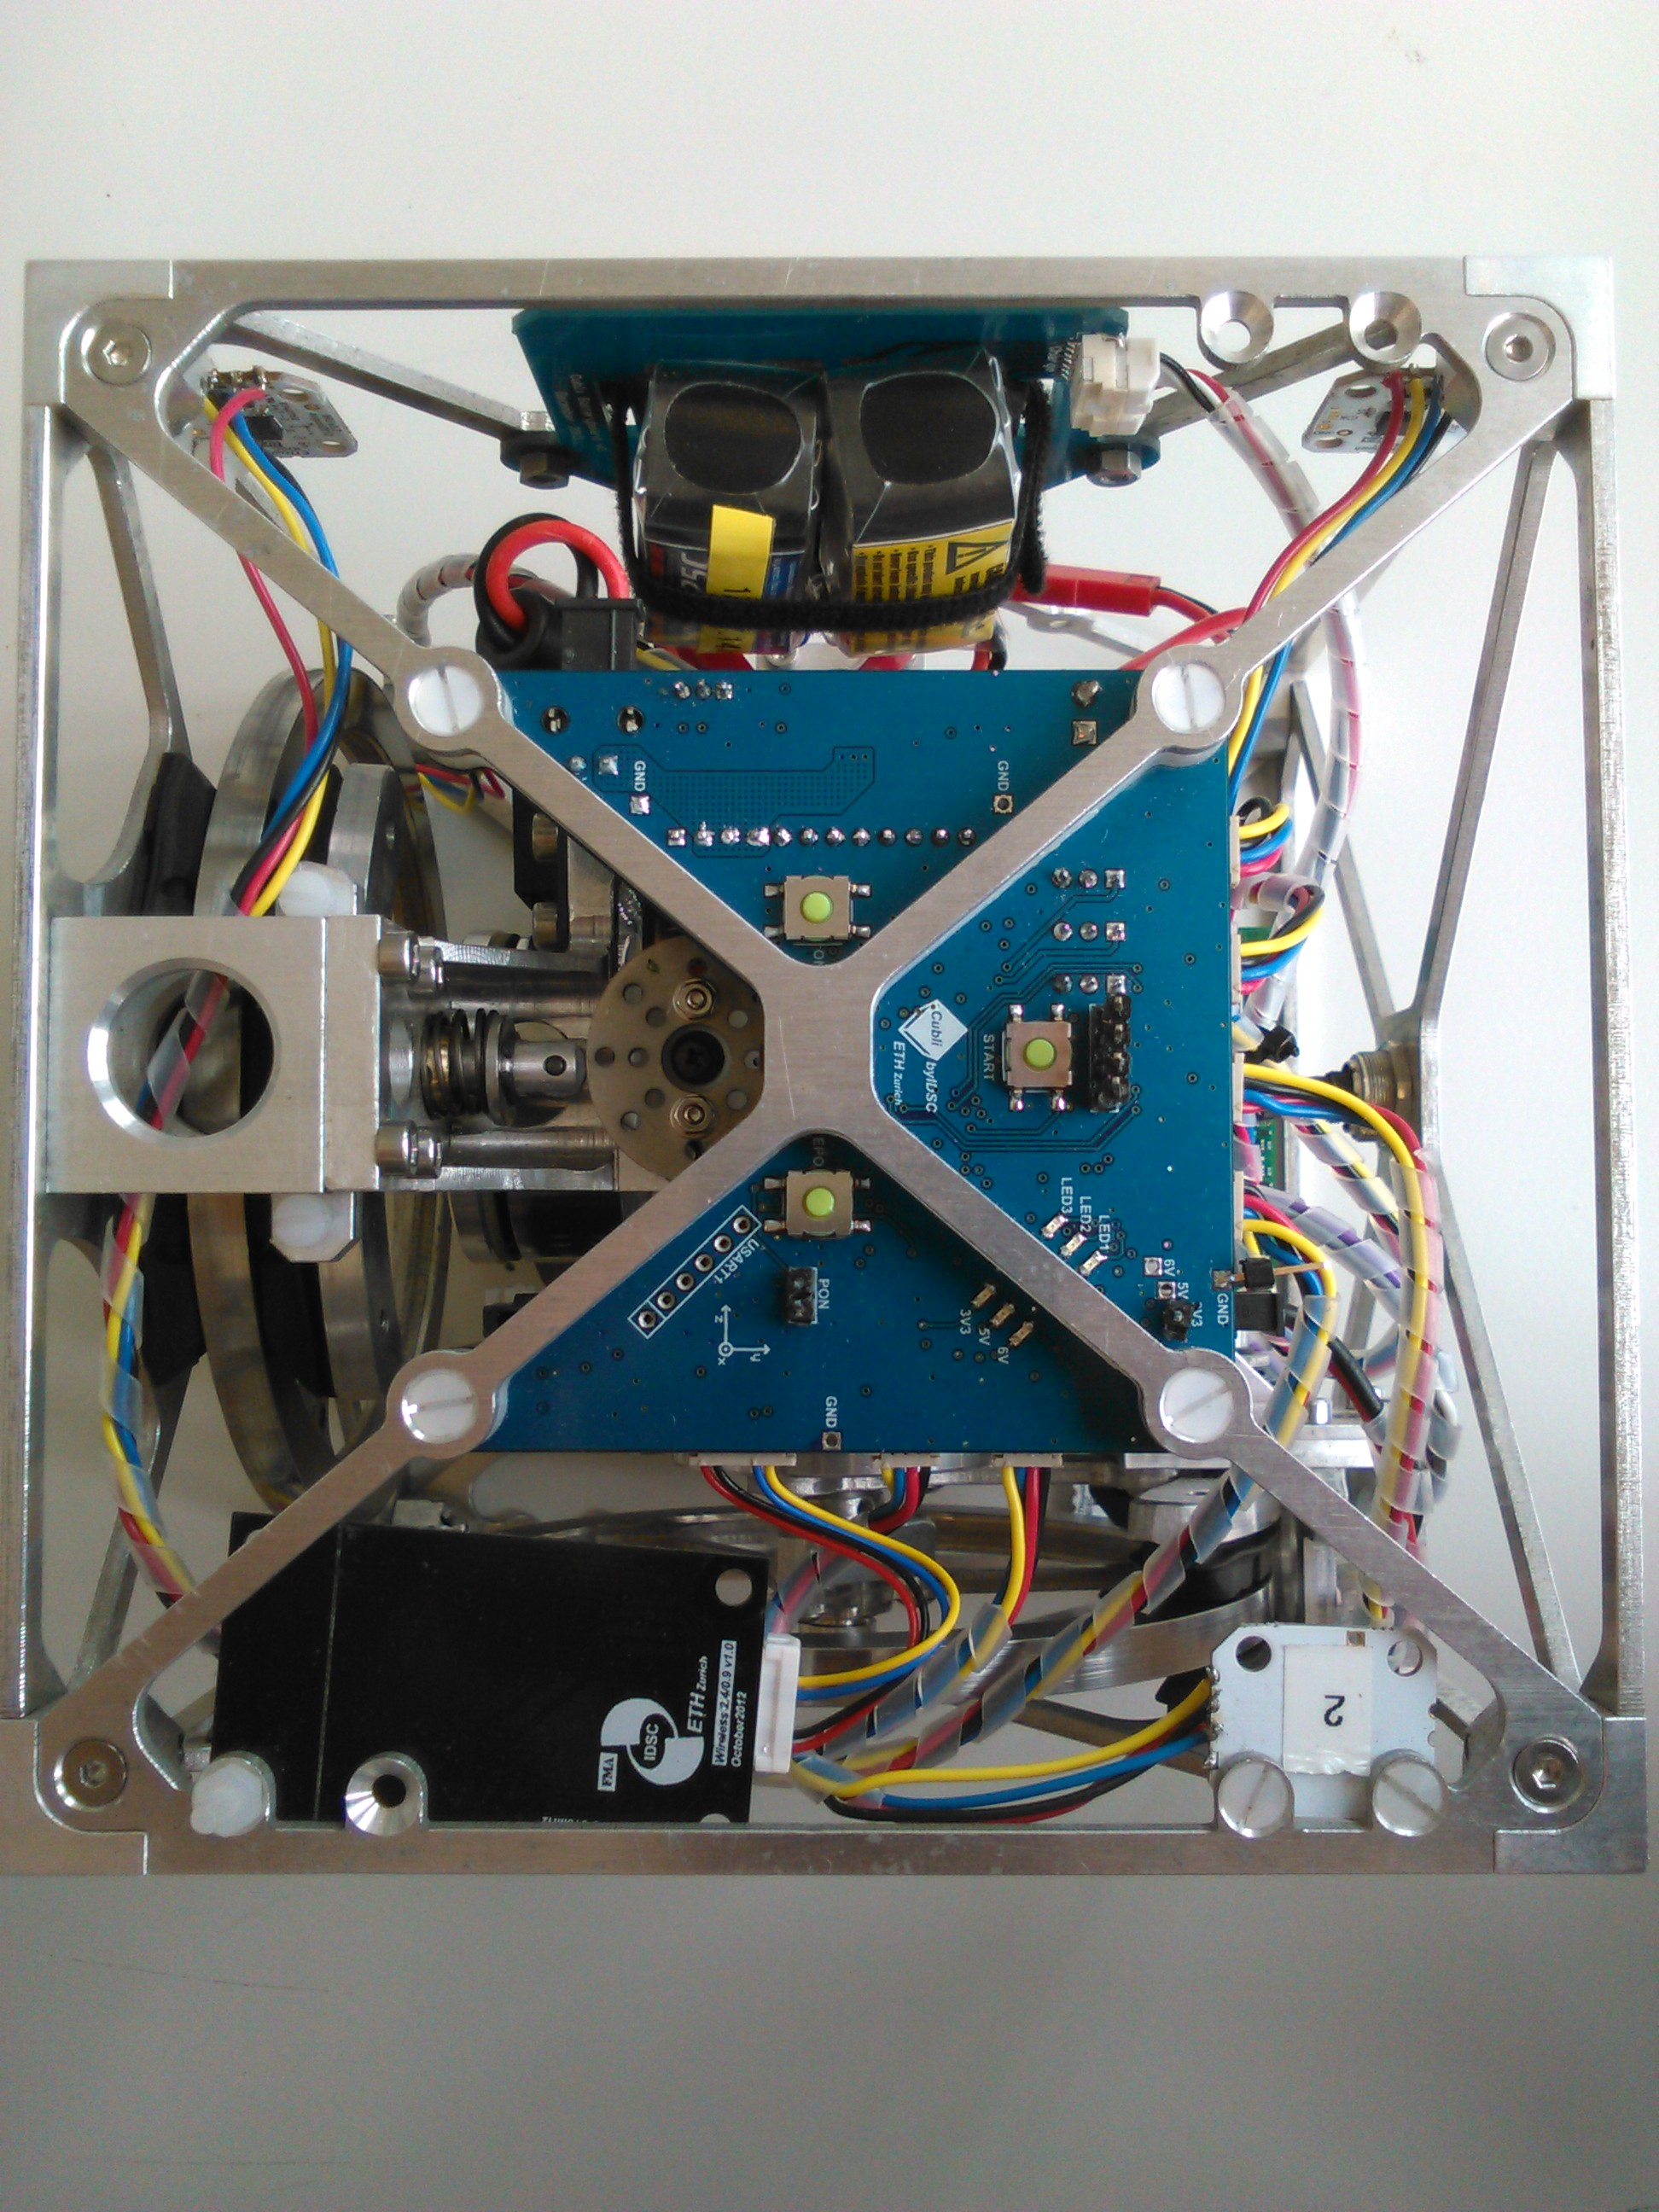
\includegraphics[width=0.75\textwidth]{img/Buttons.jpg}
   \caption{The three buttons on Cubli's main board, used for user interaction.}
   \label{img:Buttons}
\end{figure}

Though this is a very reliable interface, it can present inefficiencies. For example, it is sometimes desirable to press the mode button when Cubli is balancing, in order to have it perform an action. However, doing so upsets Cubli's balance, since pressing a button implies exerting a force on Cubli's exterior.\\

This project's proposition is to offer an alternate interface, without removing the already existing one - the buttons shall still serve their original functions. Controlling Cubli from a nearby device presents interesting challenges and possibilities, thus making for a promising aim.

\subsection{Original Communications Abilities}

Before the project was started, Cubli was already fitted with a wireless communication device, set up for one-way communication from Cubli to computer, for debugging and supervision purposes.\\

\begin{figure}[ht]
   \centering
   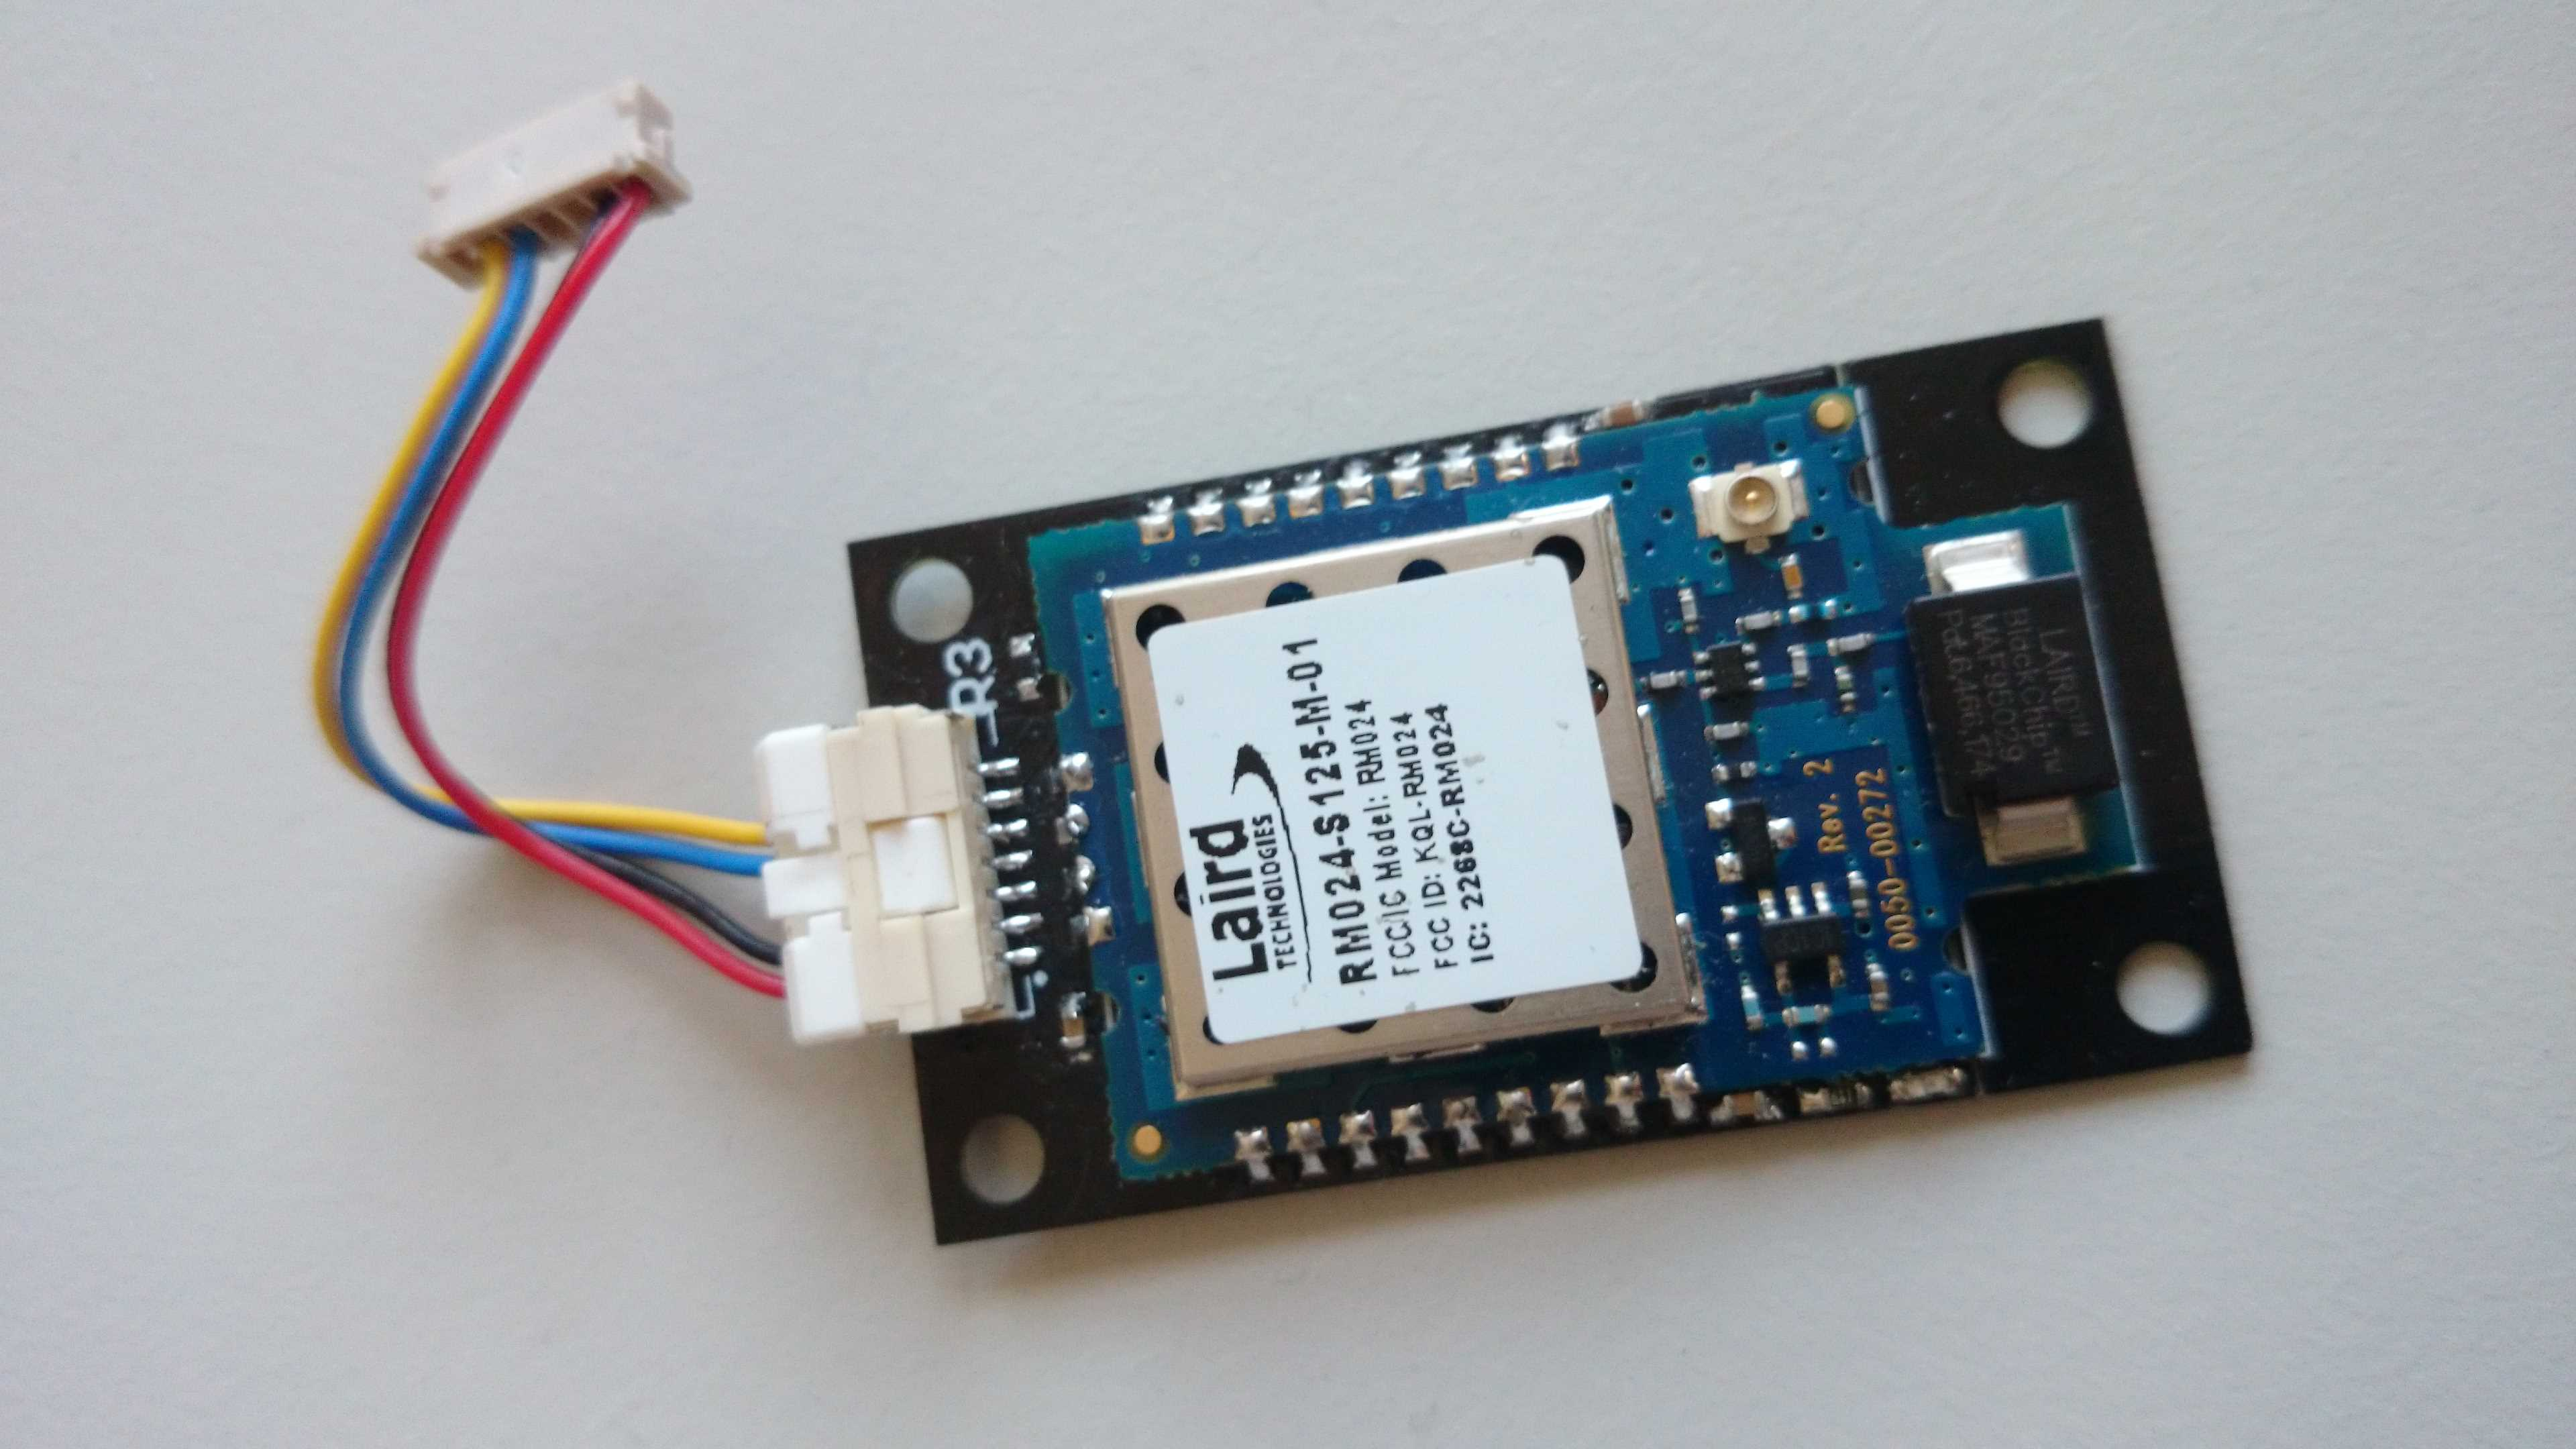
\includegraphics[width=0.75\textwidth]{img/LAIRD-radio.jpg}
   \caption{Radio used as part of the Cubli hardware.}
   \label{img:LAIRD-radio}
\end{figure}

As such it made sense to consider developping two-way communications using the already-present hardware, and the potential applications of this modification.\\ 

Because physical interaction with the robot generally hinders its ability to balance and move freely, wireless communication is a desired part of the new interface's implementation.\\

The project aims to extend the interface, but also to test Cublis ability not only to simply receive commands from the user, but also to communicate in a multilateral fashion. That is, to set the basis for smarter Cublis that can exchange information, and display responsive behavior. 

\section{Project Goals}

As the previous section outlines the original capabilities of Cubli, this section lays out the practical implementation which is sought. The implementation is meant to showcase the properties ( some of which were expressed previously ) which are:
\begin{enumerate}
\item augmented interface
\item responsiveness
\item multiple Cubli coordination
\item potential for further features
\end{enumerate}

Thus, the Cubli choreographer concept was created: An interface allowing not only for wireless control of a Cubli, but also allowing for the introduction of more independent and responsive behavior.\\

By giving the robot not straightforward commands, but more complex sequences which it needs to store and perform - acting autonomously to ensure the correct proceeding of those sequences, and reacting to failures - the interface delegates responsibility to the cube.\\

In addition, the choreographer shall be designed to interact with several Cublis at once, coordinating their actions.\\

Thus, should the concept be proved to be realizable, it will effectively showcase the desired properties outlined in the previous paragraph.